% compare current (README.md|index.html) with the file from 2 versions ago
% compare (README.md|index.html) with the one from (1|2|3|4) versions before
% compare current (README.md|index.html) with that from  ([0-9]+)-days ago

% 4/5 17:00 PDT = 4/6 9:00 JST

% 部屋を暗くする
% make the room darker 

\documentclass{sigchi}

% Use this section to set the ACM copyright statement (e.g. for
% preprints).  Consult the conference website for the camera-ready
% copyright statement.

% Copyright
\CopyrightYear{2018}
%\setcopyright{acmcopyright}
\setcopyright{acmlicensed}
%\setcopyright{rightsretained}
%\setcopyright{usgov}
%\setcopyright{usgovmixed}
%\setcopyright{cagov}
%\setcopyright{cagovmixed}
% DOI
\doi{http://dx.doi.org/10.475/123_4}
% ISBN
\isbn{123-4567-24-567/08/06}
%Conference
\conferenceinfo{UIST'18,}{October 14--17, 2018, Berlin, Germany}
%Price
\acmPrice{\$15.00}

% Use this command to override the default ACM copyright statement
% (e.g. for preprints).  Consult the conference website for the
% camera-ready copyright statement.

%% HOW TO OVERRIDE THE DEFAULT COPYRIGHT STRIP --
%% Please note you need to make sure the copy for your specific
%% license is used here!
% \toappear{
% Permission to make digital or hard copies of all or part of this work
% for personal or classroom use is granted without fee provided that
% copies are not made or distributed for profit or commercial advantage
% and that copies bear this notice and the full citation on the first
% page. Copyrights for components of this work owned by others than ACM
% must be honored. Abstracting with credit is permitted. To copy
% otherwise, or republish, to post on servers or to redistribute to
% lists, requires prior specific permission and/or a fee. Request
% permissions from \href{mailto:Permissions@acm.org}{Permissions@acm.org}. \\
% \emph{CHI '16},  May 07--12, 2016, San Jose, CA, USA \\
% ACM xxx-x-xxxx-xxxx-x/xx/xx\ldots \$15.00 \\
% DOI: \url{http://dx.doi.org/xx.xxxx/xxxxxxx.xxxxxxx}
% }

% Arabic page numbers for submission.  Remove this line to eliminate
% page numbers for the camera ready copy
% \pagenumbering{arabic}

% Load basic packages
\usepackage{balance}       % to better equalize the last page
% \usepackage{graphics}      % for EPS, load graphicx instead 
\usepackage{graphicx}      % for EPS, load graphicx instead 
\usepackage[T1]{fontenc}   % for umlauts and other diaeresis
\usepackage{txfonts}
\usepackage{mathptmx}
% \usepackage[pdflang={en-US},pdftex]{hyperref} なんかわからない
\usepackage{color}
\usepackage{booktabs}
\usepackage{textcomp}

% Some optional stuff you might like/need.
\usepackage{microtype}        % Improved Tracking and Kerning
% \usepackage[all]{hypcap}    % Fixes bug in hyperref caption linking
\usepackage{ccicons}          % Cite your images correctly!
% \usepackage[utf8]{inputenc} % for a UTF8 editor only

\usepackage{here} % [H]とするとその場所に配置されるらしい

% If you want to use todo notes, marginpars etc. during creation of
% your draft document, you have to enable the "chi_draft" option for
% the document class. To do this, change the very first line to:
% "\documentclass[chi_draft]{sigchi}". You can then place todo notes
% by using the "\todo{...}"  command. Make sure to disable the draft
% option again before submitting your final document.
\usepackage{todonotes}

% Paper metadata (use plain text, for PDF inclusion and later
% re-using, if desired).  Use \emtpyauthor when submitting for review
% so you remain anonymous.
\def\plaintitle{Bridging the Translation Gap with ExpandHelp}
% \def\plainauthor{Toshiyuki Masui, Jun Kato}
\def\plainauthor{}
\def\emptyauthor{}
\def\plainkeywords{
  Help systems; Regular expression, Input method, Generate and filter;
  ExpandHelp; GitHelp
}
% \def\plaingeneralterms{Documentation, Standardization}

% llt: Define a global style for URLs, rather that the default one
\makeatletter
\def\url@leostyle{%
  \@ifundefined{selectfont}{
    \def\UrlFont{\sf}
  }{
    \def\UrlFont{\small\bf\ttfamily}
  }}
\makeatother
\urlstyle{leo}

% To make various LaTeX processors do the right thing with page size.
\def\pprw{8.5in}
\def\pprh{11in}
\special{papersize=\pprw,\pprh}
\setlength{\paperwidth}{\pprw}
\setlength{\paperheight}{\pprh}
\setlength{\pdfpagewidth}{\pprw}
\setlength{\pdfpageheight}{\pprh}

% Make sure hyperref comes last of your loaded packages, to give it a
% fighting chance of not being over-written, since its job is to
% redefine many LaTeX commands.
\definecolor{linkColor}{RGB}{6,125,233}
% \hypersetup{%
%   pdftitle={\plaintitle},
% % Use \plainauthor for final version.
% %  pdfauthor={\plainauthor},
%   pdfauthor={\emptyauthor},
%   pdfkeywords={\plainkeywords},
%   pdfdisplaydoctitle=true, % For Accessibility
%   bookmarksnumbered,
%   pdfstartview={FitH},
%   colorlinks,
%   citecolor=black,
%   filecolor=black,
%   linkcolor=black,
%   urlcolor=linkColor,
%   breaklinks=true,
%   hypertexnames=false
% }

% create a shortcut to typeset table headings
% \newcommand\tabhead[1]{\small\textbf{#1}}

% End of preamble. Here it comes the document.


\def\GH{\textsf{GitHelp}}
\def\SB{\textsf{Scrapbox}}
\def\EH{\textsf{ExpandHelp}}
\def\GIT{\texttt{git}}
\long\def\tt#1{\texttt{#1}}
\long\def\stt#1{\texttt{\fontsize{9pt}{0pt}\selectfont{#1}}}
\long\def\sf#1{\textsf{#1}}
\long\def\ssf#1{\textsf{\fontsize{9pt}{0pt}\selectfont{#1}}}
\long\def\qtt#1{``\tt{#1}''}   % quote tt
\long\def\sqtt#1{``\stt{#1}''} % small quote tt
\long\def\qsf#1{``\sf{#1}''}
\long\def\sqsf#1{``\ssf{#1}''}
\long\def\qit#1{``\textit{#1}''}
\long\def\smallfont{\fontsize{9pt}{0pt}\selectfont}

\begin{document}

\title{\plaintitle}

\numberofauthors{3}
\author{%
%  \alignauthor{Toshiyuki Masui \\
%    \affaddr{Keio University}\\
%    \affaddr{Fujisawa, Japan}\\
%    \email{masui@pitecan.com}}\\
%  \alignauthor{Jun Kato\\
%    \affaddr{AIST}\\
%    \affaddr{Tsukuba, Japan}\\
%    \email{junkato}}\\
  \alignauthor{-- \\
    \affaddr{--}\\
    \affaddr{--}\\
    \email{--}}\\
  \alignauthor{--\\
    \affaddr{--}\\
    \affaddr{--}\\
    \email{--}}\\
}

\maketitle

\begin{abstract}
  We introduce a flexible command translation framework that can generate
  a complex command string from vague keywords
  given by the user.
  %
  % Although intuitive GUI are 
  % command-line interface (CLI) is still widely used everywhere,
  %
  When people use computers to perform tasks,
  there is often a huge mismatch between the users' intention
  and required actions.
  % the language and vocabularies used for the task are completely different.
  %
  For example, when a Chinese person wants to ``房間暗一点'' (make the room darker),
  % he may have to translate his intention into an English expression ``make the room darker'',
  he may have to find that he should ``turn off the ceiling light'' for the task,
  translate it to a required action ``toggle the wall switch''
  or a command like ``\tt{\$ iot clight 0}''.
  %
  % When a user wants to ``make the room darker'',
  % he should translate it to a real action like ``turn off the ceiling light''.
  % To do so,
  % he may have to ``toggle the wall switch''
  % or issue a command like ``\tt{\$ iot ceilinglight 0}''.
  % If the user is a Chinese speaker, he might have to translate his intention
  % ``房間暗一点'' into ``make the room darker'',
  % ``turn off the ceiling light'', 
  % ``toggle the wall switch'',
  % and finally to a command like ``\tt{\$ iot ceilinglight 0}''.
  %
  There is a huge gap between ``房間暗'' and ``\tt{\$ iot clight 0}'', and
  people are perpetually suffering from such multi-level ``\textit{translation gaps}''.
  Translation gaps exist even for experienced computer users, but
  they are serious for vast amount of people
  whose mother languages are far from the command syntax required for
  handling computers.
  %
  We propose a simple and flexible translation framework
  {\EH} that can be used in various situations
  where such translation is necessary.
  We show how our framework can be used
  in the {\GH} system
  with which a user can easily generate complex {\GIT} commands
  from fragments of users' intentions in various languages.
\end{abstract}

\category{H.5.m.}{Information Interfaces and Presentation
  (e.g. HCI)}{Miscellaneous}

% \category{See
%   \url{http://acm.org/about/class/1998/} for the full list of ACM
%   classifiers. This section is required.}{}{}

\keywords{\plainkeywords}

\section{Introduction}

When people want to perform a task using modern artifacts,
people frequently find difficulty handling them properly.
%
Even when manuals and help documents are provided,
people don't use them\cite{Novick:2006:WDP:1166324.1166329}
partly because of the vocabulary problem\cite{Furnas:1987:VPH:32206.32212}.
%
% Twitterでのアンケート: 80\% が全然使わない
% https://gyazo.com/2dd525388cce34c916638f51bad386c7
% 
% やりたいと思ったことがすぐできればどれほど嬉しいことか
% そもそも検索や翻訳が必要なものであるならそれを楽にすればよい
%
We should translate our vague intentions in our brain into actions required for the artifacts.
When we want to watch a movie, we may pick up a DVD disk, put it into a
DVD player, push the play button, and set up the audio and the monitor.
When we feel thirsty, we may go to the kitchen, pick up a glass, and
turn the faucet on to fill the glass with water.
In either of these cases, there is a tremendous gap
between the user's intentions and required actions.
All the living creatures are seemingly performing such translations
between intentions and actions without difficulty, but
in the modern world, people are suffering from
serious gaps between what they want to do and what they have to do.

Even when people almost know what they have to do,
it is often not easy for them to perform the task without confusion.
Even when people know that they can watch a movie on the Internet,
finding a movie and playing it is a difficult task for people without experiences.
It would be nicer if they could watch a movie
just by showing a fragment of the title or attributes of the movie.

% We can use search engines to find clues for performing the tasks, but
% it is not always easy for people in the world, since they may have
% to use different languages to look for the information.

We propose a simple, flexible and powerful
translation framework {\EH}, with which users can generate a complete
command string from fragments of users' vague intentions.
%
We use a database consisting of pairs of
the description of the task that users want to perform (e.g. 房間暗一点)
and
the actual command string required by the system (e.g. \tt{\$ iot clight 0}).
Descriptions can be written in any natural language using regular expressions
and the database are shared on the Wiki pages and can be edited by any user
who wants to improve the database.

% やりたいことの[* 平易な表現と実行コマンドの組を用意]して[* 共有]しておいて、[* 簡単に検索/実行]できるようにする
% 表現は[* 何語で書いてあってもかまわない]
% 例えば映画作品見たいならAmazon PrimeとNetflix両方に作品があったりする
% コマンドの例でいえば何をどの順番でパイプするかいろいろ選択肢がありうる
% 全部出てくれると便利ですね(自分の知らなかったコマンド記法が学べたりする)
% いろんな候補は出ます [増井俊之.icon]
% 「Amazonでゴジラを見る」「Netflixでゴジラを見る」みたいに
% コマンドの勉強になる とは思っています [増井俊之.icon]
% そういう話は記述した方がいいかも
% `@{2 days ago}`なんて記法を知ってる人は見たことなし [増井俊之.icon]
% 今は自力で打てるようになった!
% これを[* IMEみたいなインタフェースで利用する]
% ちなIMEはアジアでは常識ね
% [* データはWikiで共有しておいて誰でも追加/修正できる]
% 自分のやり方を定義してもいい

Contributions of this paper are as follows:

\begin{enumerate}
% 各種技術を組み合わせた翻訳支援というパラダイムの提案
\item Introduction of ``\textit{translation paradigm}'' for
  generating a correct command to an artifact from
  the user's vague intention.
\item Flexible dynamic help extraction algorithm
  ``\textit{generate and filter}''
  using regular expressions.
% そのための柔軟なインフラ (ExpandHelp)
% \item IME-like command entry interface
% やりたいことを実行するインタフェース (IME的なもの)
\item Help data sharing infrastructure for the above strategy.
% 共有/編集しやすい正規表現DSLとそのインプリ(Scrapbox+)
% \item これが唯一の解決法ではないが、こういう考え方がポピュラーになって欲しい
\end{enumerate}

\section{Example: GitHelp}

We implemented the {\GH} system
with which a user can translate his vague intention in various languages
into a complete {\GIT} command
using the {\EH} framework.

% \subsection{Entering a command}

We assume that the user uses \tt{bash} for his software
development activities.
% 
When a user wants to compare the latest \stt{README.md} file
with the same file from 2 versions before,
he might try to use {\GIT} with an option
``{\smallfont\verb|HEAD^^|}''
for specifying the old version.

\begin{figure}[h]
  {\smallfont
  \verb|$ git diff HEAD^^ README.md|
  \par
  \verb|$|
  }
  \caption{Invoking \stt{git diff}.}
  \label{gitdiff}
\end{figure}

% \begin{quotation}
%   {\smallfont
%   \verb|$ git diff HEAD^^ README.md|
%   \par
%   \verb|$|
%   }
% \end{quotation}

However, nothing happens here because
\verb|HEAD^^|
specifies a file included in the older commit,
and the command in figure \ref{gitdiff} only compares the
\stt{README.md} with the file included in an old commit, where
\stt{README.md} might not have changed since then.

If {\GH} is installed,
the user can type a special shortcut key
% (e.g. \tt{Cmd-Ctrl-G})
to invoke {\GH} after typing \sqtt{git RE 2} to see how he can
perform the task.

\begin{figure}[h]
  % 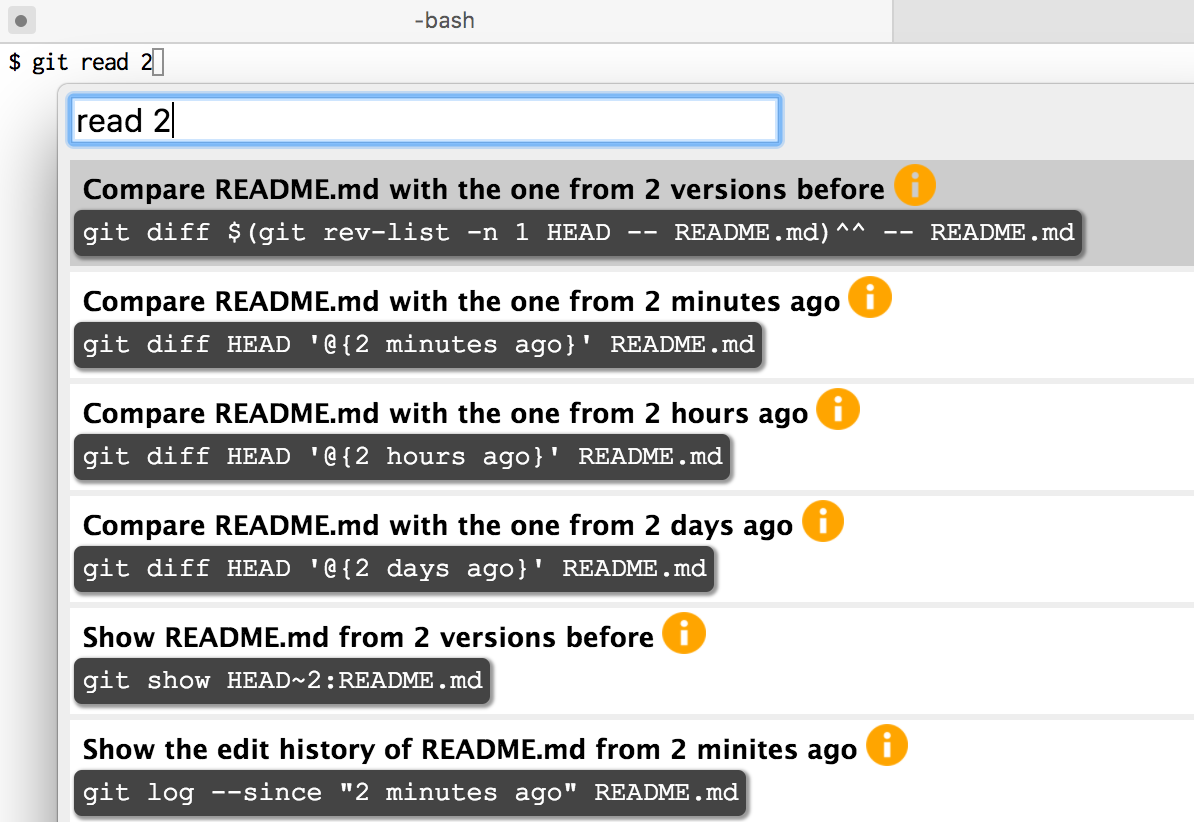
\includegraphics[width=9cm,bb=0 0 1194 822]{figures/example1.png}
  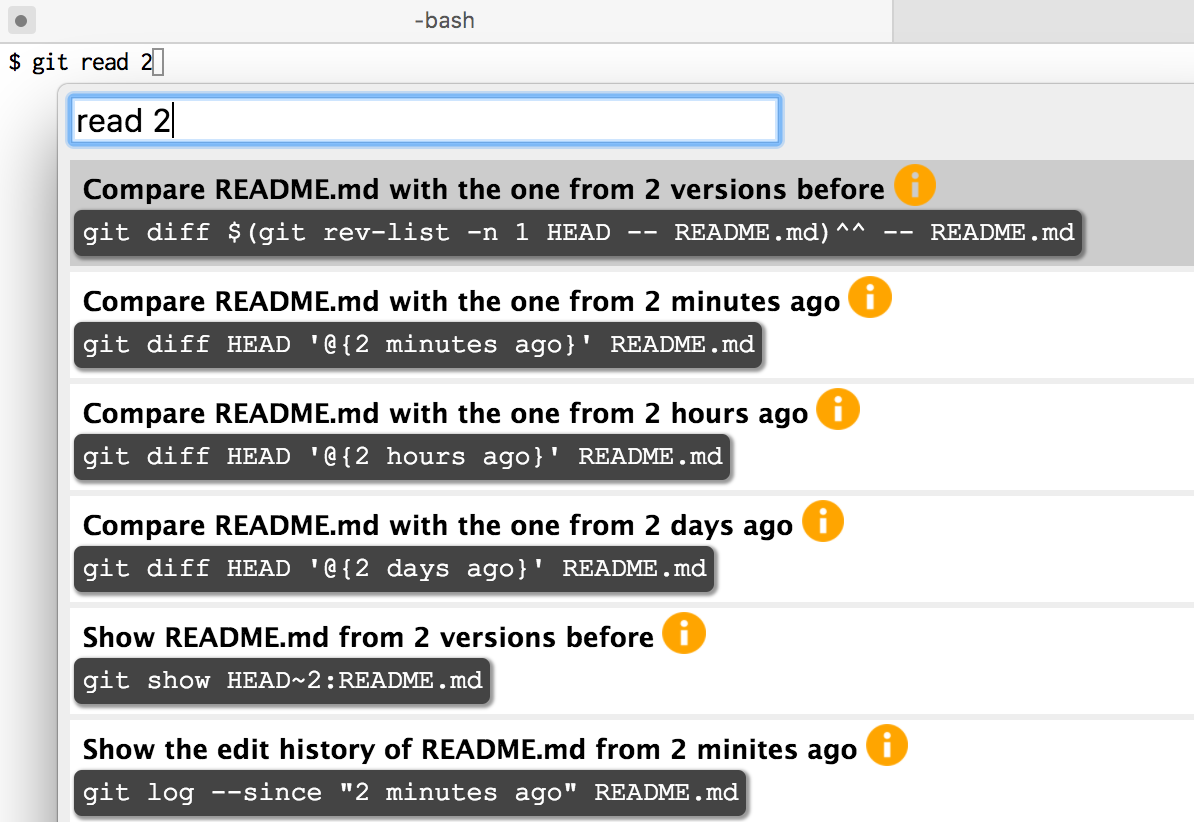
\includegraphics[width=9cm,bb=0 0 900 600]{figures/example1.png}
  %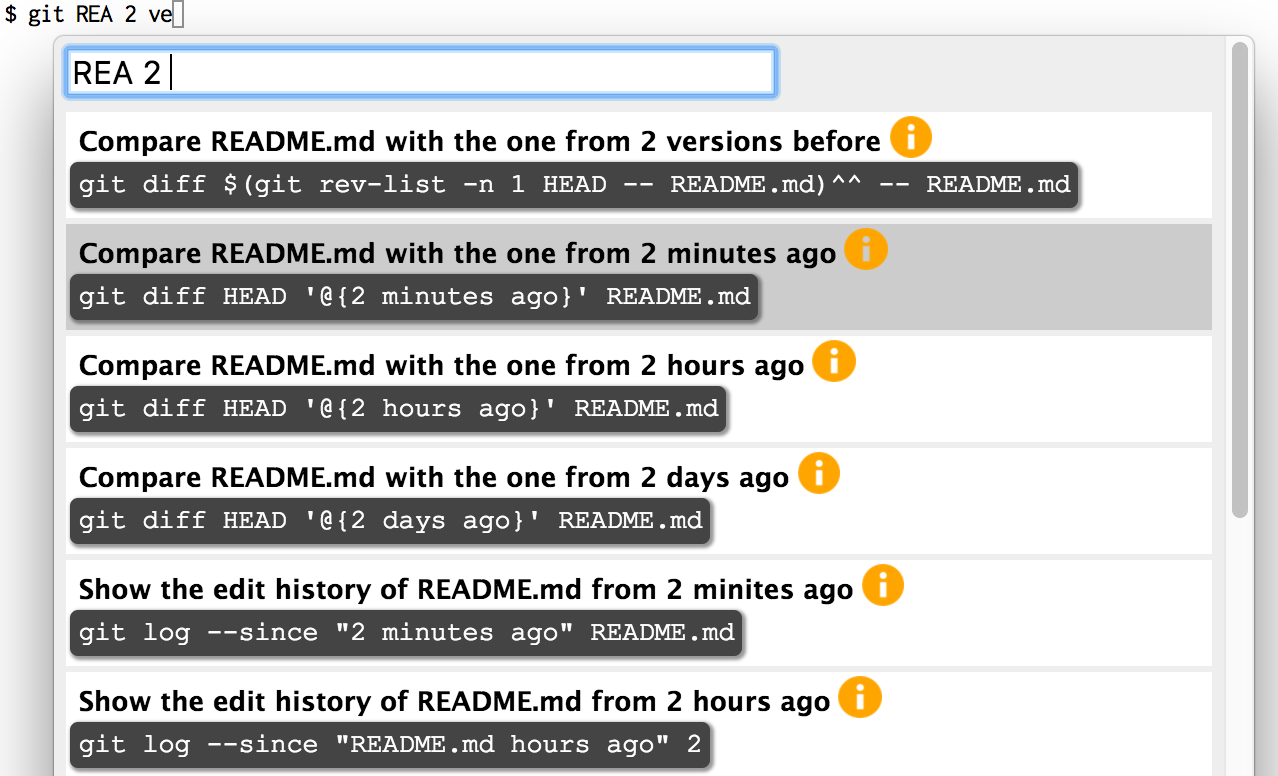
\includegraphics[width=9cm,bb=0 0 1000 600]{figures/githelp_e2.png}
  \caption{Invoking {\GH} after typing \stt{git read 2}.}
  \label{example1}
\end{figure}

Here, various candidate entries with
descriptions and command strings are listed,
just like text input support systems for non-English languages.
One of the entries says
``\ssf{Compare} \stt{README.md} \ssf{with the one from 2 versions before}'',
and if the user thinks that's what he wants to do,
he can select the entry by typing arrow keys and type the enter key.
Then the user's input string is replaced by the right command string
that satisfies the user's need.

A description like \sqsf{2 days ago} is also shown in the candidate list
of Figure \ref{example1}.
This means that the user can use the same string \sqtt{git RE 2}
for getting the information of \stt{README.md} file of the day before yesterday.
The generated argument
``{\smallfont\verb|@{2 days ago}|}'',
may not be familiar to most {\GIT} users,
but users can perform this task only by giving \sqtt{RE} and \sqtt{2}
without knowing the correct syntax of this option.

When the user types a special shortcut key
after typing \sqtt{git sh reed 3},
entries related to \stt{README.md} file are listed because
\sqtt{reed} is close to \sqtt{README.md}.

\begin{figure}[h]
  %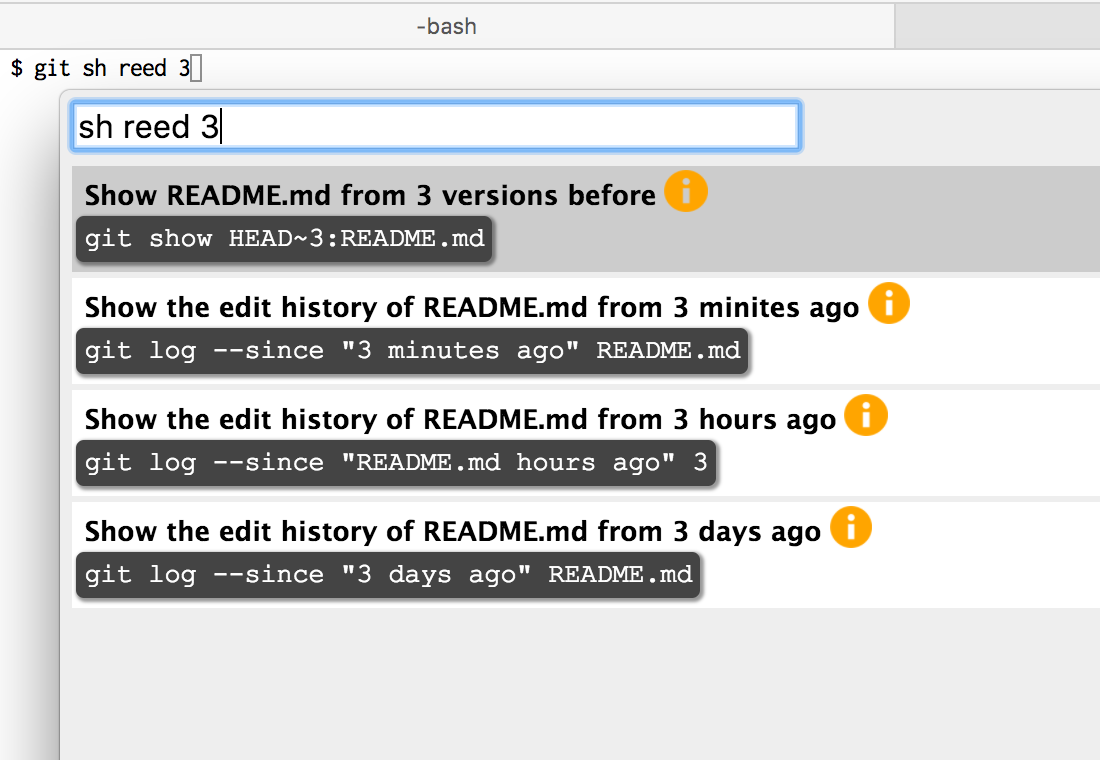
\includegraphics[width=9cm,bb=0 0 1100 760]{figures/example2.png}
  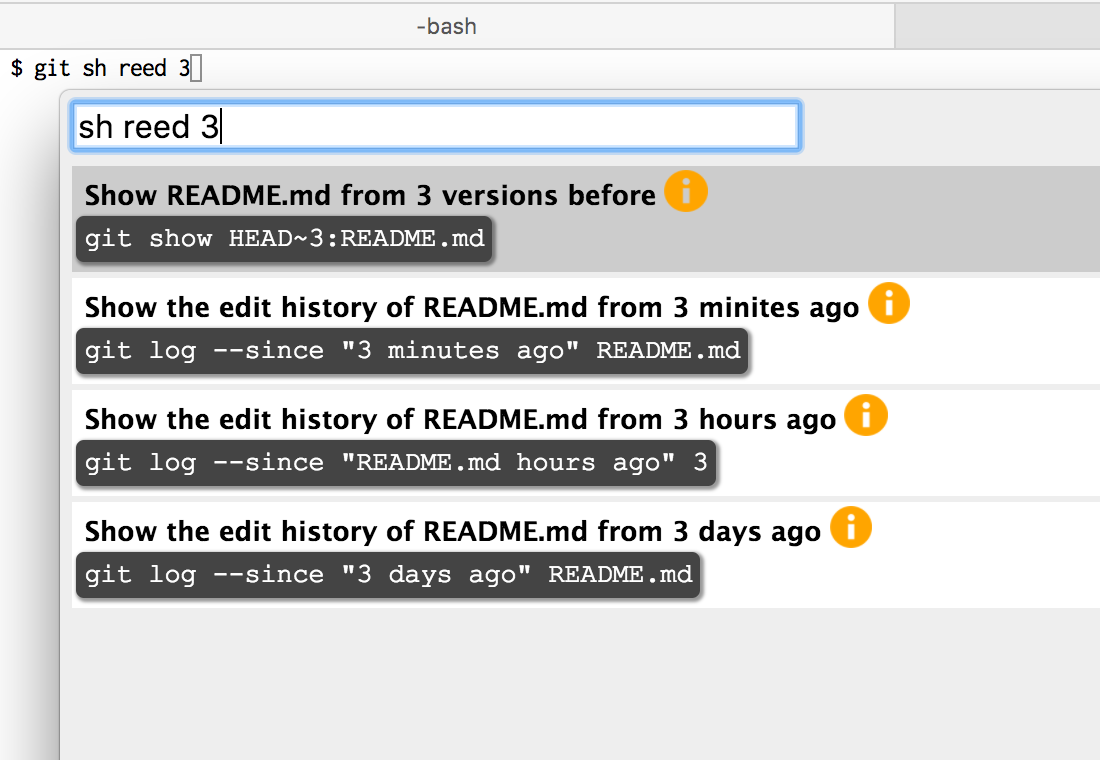
\includegraphics[width=9cm,bb=-100 0 800 550]{figures/example2.png}
  \caption{Invoking {\GH} after typing \stt{git sh reed 3}.}
  \label{example2}
\end{figure}

A Japanese {\GIT} user can do the same thing just like
English-speaking users (Figure \ref{example3}).
He can use the term \qtt{表}, etc. to find how he can perform the job.

\begin{figure}[t]
  % bb=0 0 1290 866
  % \includegraphics[width=12cm,bb=-100 -100 1190 766]{figures/githelp1.png}
  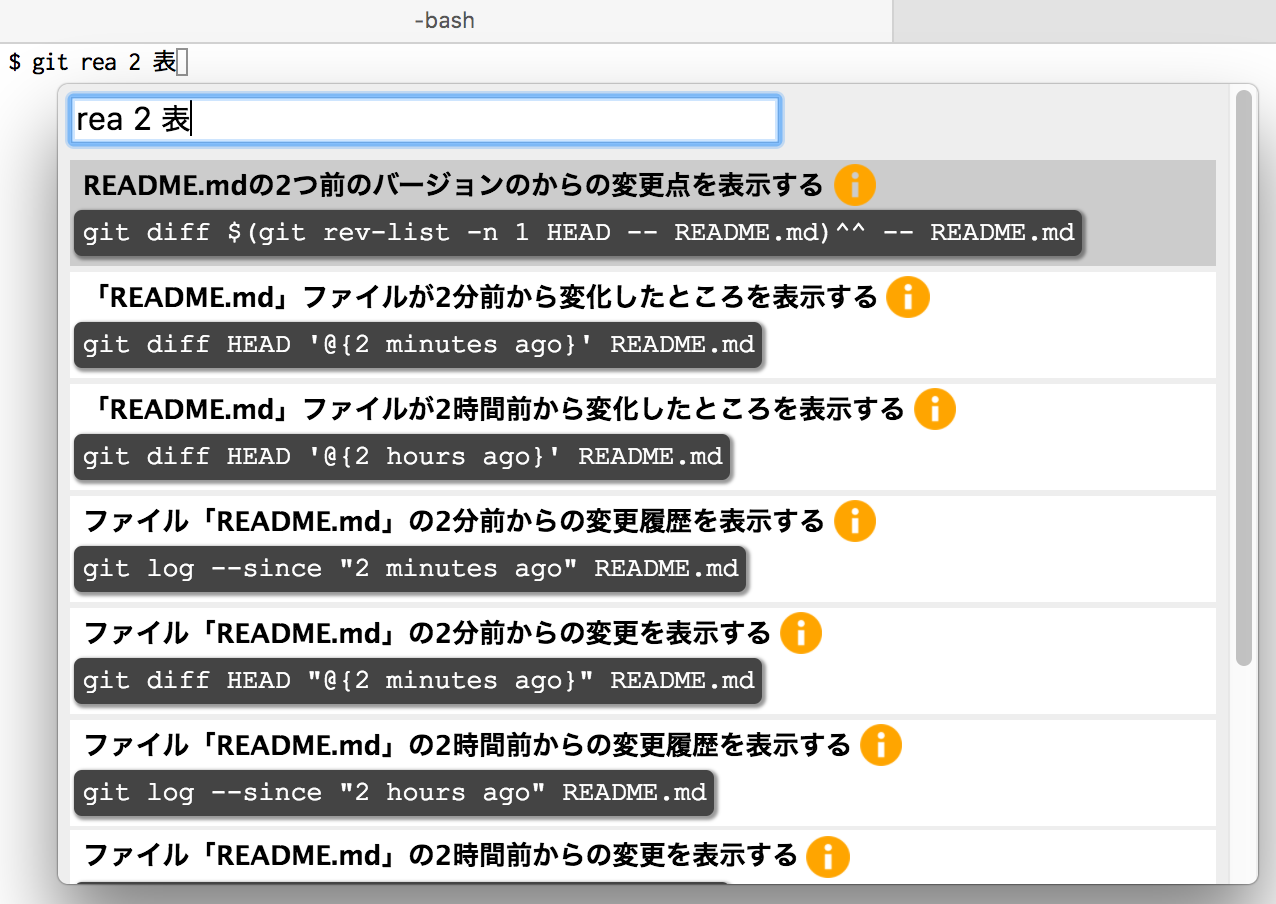
\includegraphics[width=12cm,bb=-100 -100 1190 766]{figures/example4.png}
  \caption{Invoking {\GH} in Japanese environment.}
  \label{example3}
\end{figure}

If the user wants to know more about the command line,
he can click the
\raisebox{-2pt}{
\includegraphics[height=11pt,bb=0 0 200 200]{figures/info-xxl.png}}
button and see the Wiki page shown in Figure \ref{scrapboxpage}.
The user can edit the page if he wants to add information or finds an error.
In this page, description part is preceded by a ``\texttt{\$}'' symbol and
the command part is preceded by ``\texttt{\%}''.


\begin{figure}[t]
% \centerline{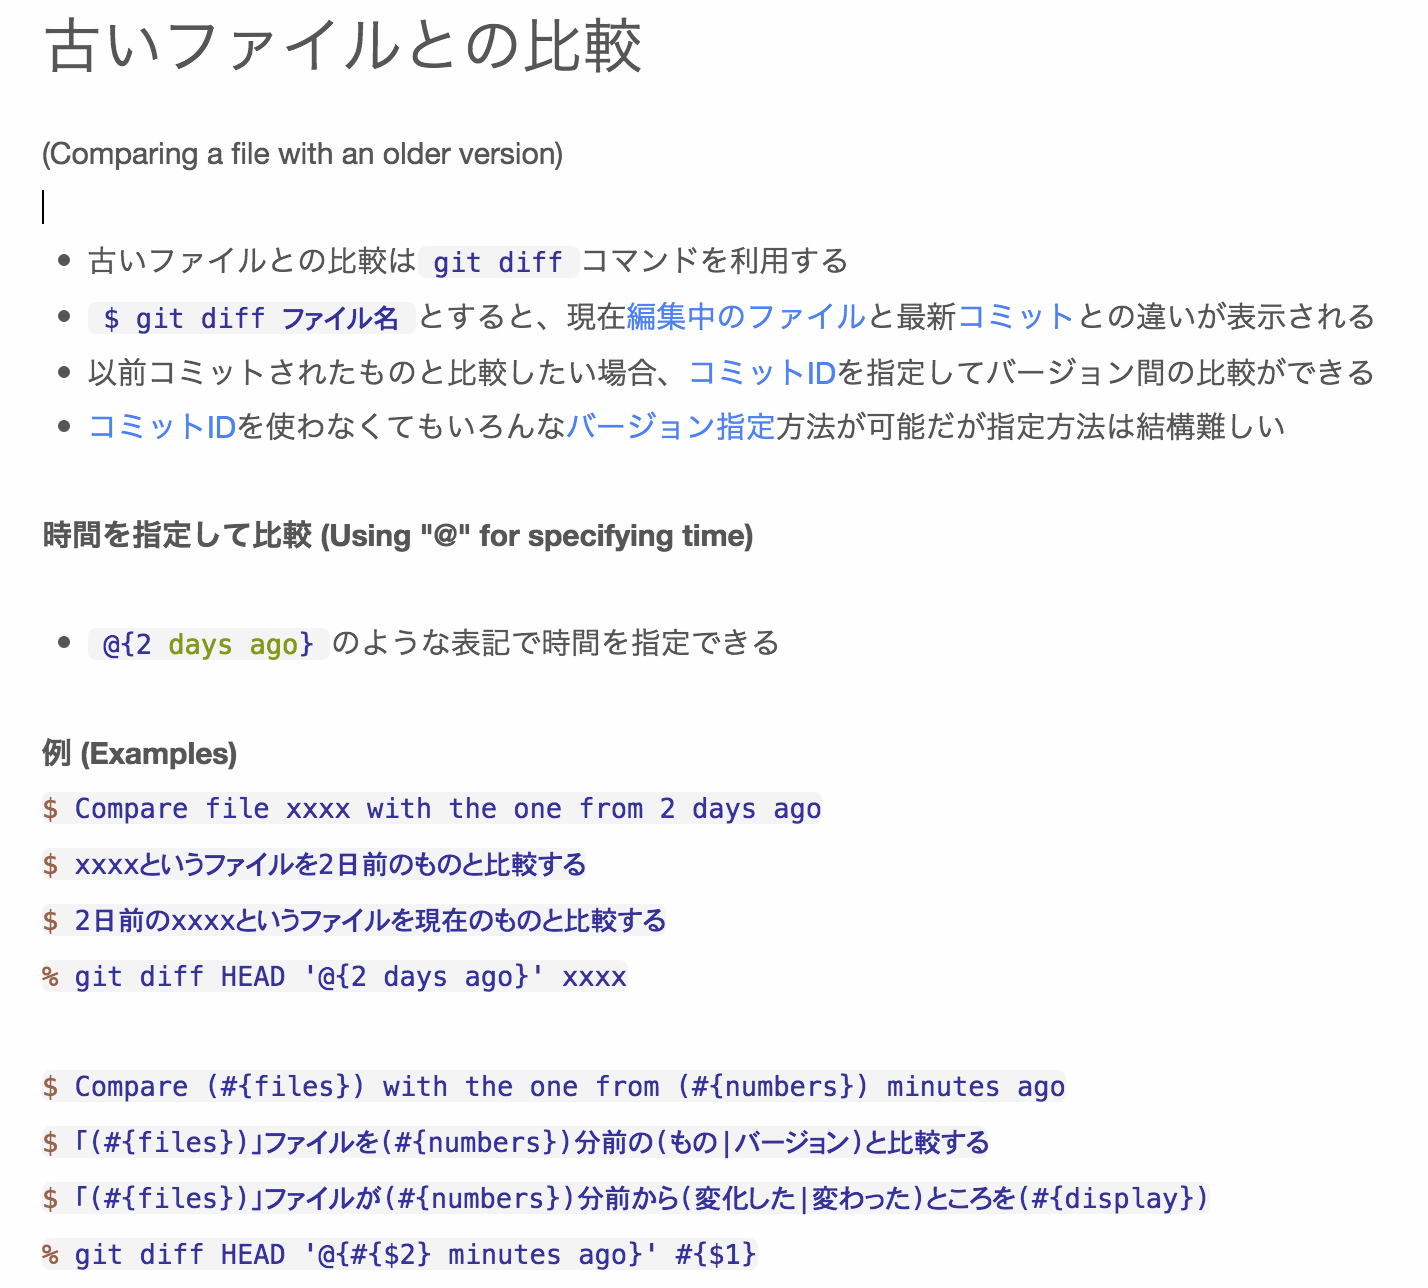
\includegraphics[width=100mm,bb=0 0 1428 1288]{figures/scrapbox1.png}}
  \centerline{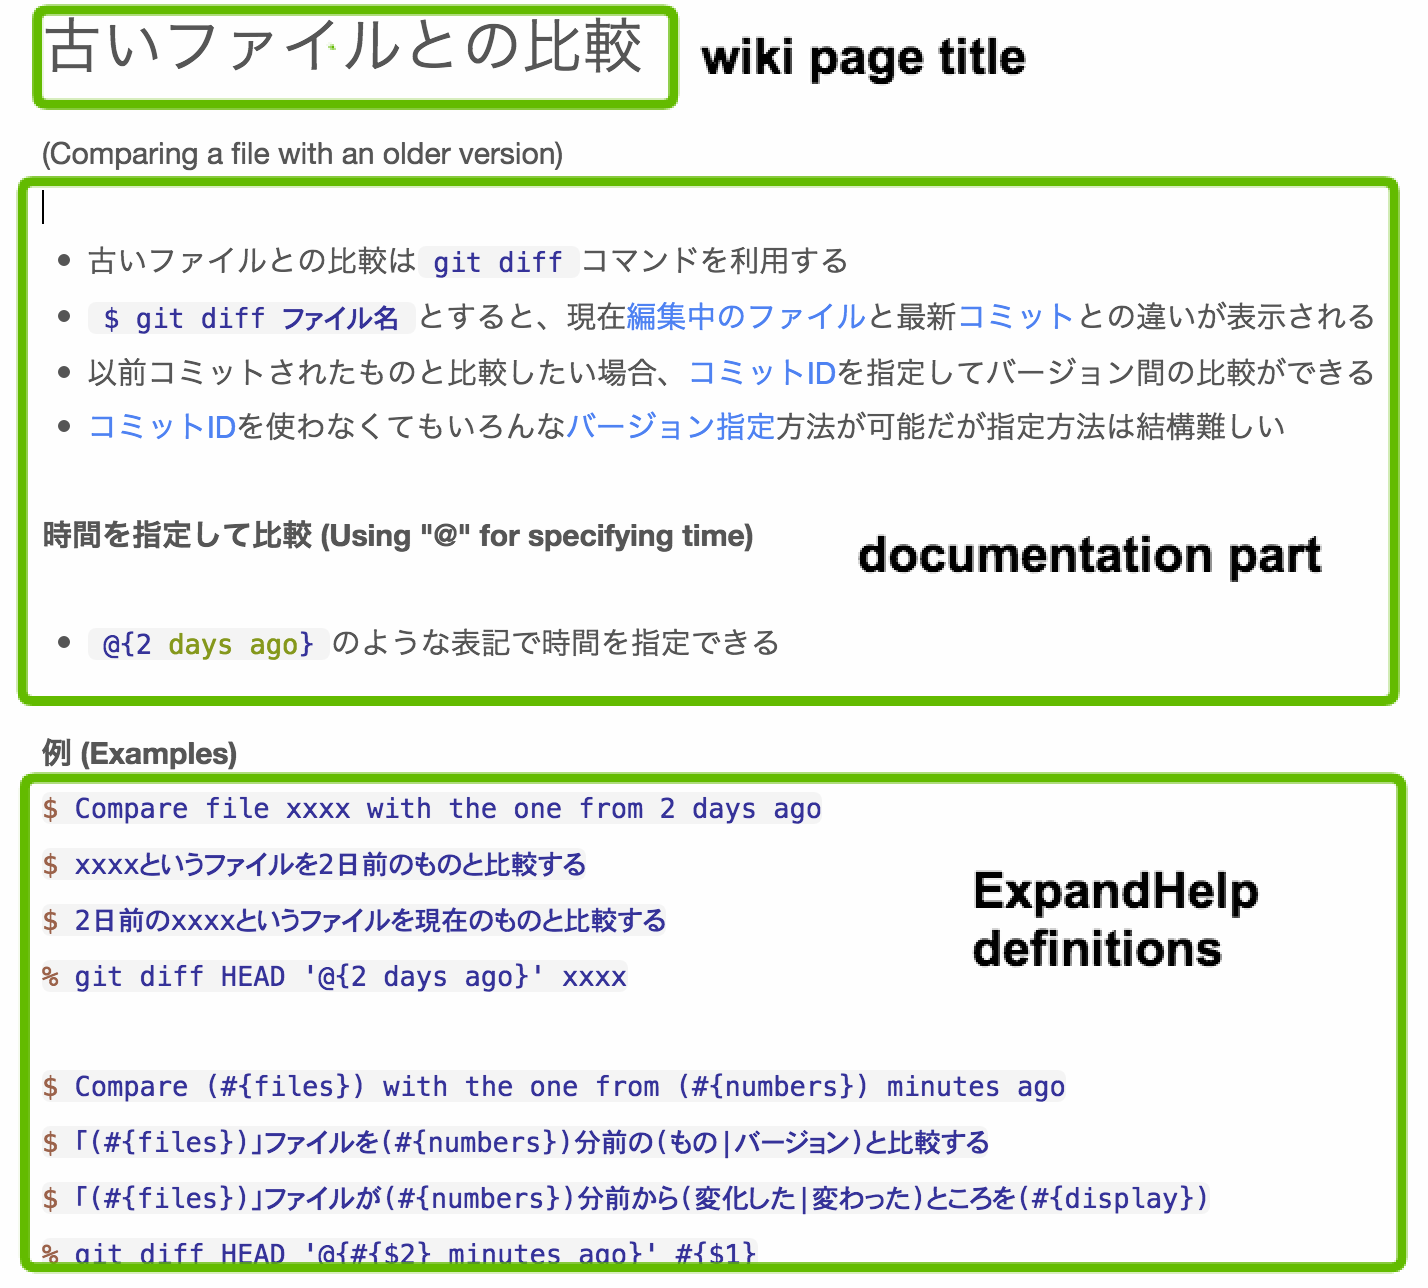
\includegraphics[width=100mm,bb=-50 -50 1100 950]{figures/scrapbox3.png}}
  \caption{A {\SB} page for \tt{git diff}.}
  \label{scrapboxpage}
\end{figure}

\section{Implementation}

\subsection{ExpandHelp}

A flexible help data retrieval mechanism ``{\EH}'' is used in {\GH}.
%
Help data used in {\EH} are provided as a set of data entries
consisting of a regular expression that represents description of the help entry
and a corresponding command pattern string.
A description string is used to produce natural language texts
that are easily understandable by users,
while command patterns represents the generated command string
corresponding to the description.
%
For example, a help entry for showing the difference between
current file and older file can be defined like this:

\begin{quote}
  \textbf{description}: \\
  \stt{Compare (\#\{files\}) with the one from (1|2|3|4) versions before}\\
  \textbf{command}: \\
  {\smallfont\verb|git diff $(git rev-list -n #{$2} HEAD -- #{$1})^|} \\
  {\smallfont\verb| -- #{$1}|}
\end{quote}

Special symbols like \stt{\#\{files\}} in the description part is expanded to
the list of filenames like \stt{README.md|index.html}.
The first regular expression, the description part,
is for generating texts like
\sqsf{Compare README.md with the one from 1 versions before}, 
\sqsf{Compare index.html with the one from 2 versions before}, etc.,
and the second part, command part,
is used to generate a command to execute a {\GIT} command.
In the first example, \sqsf{README.md} and \sqsf{1}
match the first and second parentheses of the regular expression, and
these values are assigned to \tt{\$1} and \tt{\$2}
for the command part, generating a command
``{\smallfont\verb|$ git diff $(git rev-list -n #{$2} HEAD -- #{$1})^|}
{\smallfont\verb|-- #{$1}|}''.

The description part can be written in any natural language.
For example,

\begin{quote}
  \stt{(\#\{files\})を(1|2|3|4)個前のものと比較する}
\end{quote}
  
can be used for Japanese users.
In this case,
\sqsf{README.mdを1個前のものと比較する},
\sqsf{README.mdを2個前のものと比較する}, etc.
are used for the matching.

%% \subsection{(section written for GitHelp)}
%% 
%% {\EH} is a general-purpose flexible help generation system
%% that has the following characteristics.
%% 
%% \begin{itemize}
%% \item Use description-execution pairs for the translation
%% \item Standard regular expression is used for the specification of the description
%% \item The specification RegExp is expanded and filtered by the user's input string
%%   real-time
%% \end{itemize}
%% 
%% An example of the desc-exec pair can be the following:
%% 
%% \begin{verbatim}
%%   (delete|remove) a (#{file})
%%   /bin/rm $2
%% \end{verbatim}
%% 
%% ``remove \verb|README.md|''
%% into
%% ``\verb|rm README.md|
%% 
%% First, the spec like \stt{\#\{file\}} is expanded to a list of filenames like
%% \verb+README.md|Makefile|test.c+,
%% and the spec string becomes
%% ``\verb+(delete|remove) a file (README.md|Makefile|test.c)+''.
%% Then this regular expression is expanded to all the possible string that match this regexp like
%% \begin{verbatim}
%% delete a file README.md
%% remove a file README.md
%% delete a file Makefile
%% remove a file Makefile
%% ...
%% \end{verbatim}
%% 
%% And then all these strings are compared with the user's specification like
%% ``\verb|del REA|'',
%% and if a match is found,
%% this is translated to
%% ``\verb|delete file README.md|''.
%% 
%% If ``\verb|destroy|'' should also be used for the spec,
%% the spec can be modified to 
%% \stt{(delete|remove) a (\#{file})}.
%% 
%% Any kind of specs in any language can be used for the specification.
%% For example,
%% 
%% \begin{verbatim}
%%   \#{file}を(消す|消去する)
%%   /bin/rm $1
%% \end{verbatim}
%% 
%% can be  used for Japanese users, who might want to delete
%% one of the files by specifying ``消す''.
%% (消す means 'delete' in Japanese).

\subsubsection{Generating help menu entries}

Finding appropriate entries from the (possibly huge) help document space is
performed in two steps.
First, a state transition diagram is generated from the regular expressions
used in the descriptions.
Second, all the description strings are generated by expanding the regular expression
into a tree, and filter the generated strings by the pattern specified by the user.
Efficient pattern matching is performed every time a new description text is generated,
and only the best-matched descriptions are shown to the user as menu entries.
We call this the ``\textit{generate-and-filter}'' technique,
and we will describe the details later.

\paragraph{Phase 1: Generating a state transition diagram from a regular expression}

Regular expressions are widely used for finding patterns in text strings
in modern programming languages and in the Unix environment.
In {\EH}, we use regular expressions for
generating various patterns of descriptions from a short specification.
For example, we use a short regular expression
\sqtt{(remove|delete|erase) (data|file)}
for representing expressions like
\sqsf{remove data},\sqsf{erase file}, etc.

Converting a regular expression to a state transition machine is a
straightforward task.
When we have a regular expression
\sqtt{Compare (README.md|index.html|package.json) with the one (1|2|...|10) versions before}, 
we can convert it into a state transition diagram
shown in Figure \ref{statemachine1}.

\begin{figure}[htb]
\includegraphics[width=90mm,bb=0 0 571 126]{figures/statemachine.pdf}
\caption{State transition diagram for a \stt{git} command description.}
\label{statemachine1}
\end{figure}

By traversing the nodes and links in this state machine,
we can generate the following description texts.

\begin{quote}
\small
\ssf{Compare README.md with the one 1 versions before} \\
\ssf{Compare index.html with the one 1 versions before} \\
...\\
\ssf{Compare package.json with the one 10 versions before}\\
\end{quote}

\paragraph{Phase 2: Generating texts from a state transition diagram}

Using the state transition diagram shown in Figure \ref{statemachine1},
{\EH} generates all the strings represented in the regular expressions,
and filter them by the pattern provided by the user.

We can generate texts from a state transition diagram by traversing nodes one by one.
Starting at the start node
(\raisebox{-2pt}{\includegraphics[height=10pt,bb=0 0 40 40]{figures/startnode.pdf}})
in Figure \ref{statemachine1},
we can visit other nodes via edges and generate a tree of generated texts
shown in Figure \ref{gentree1}.
After visiting the initial node
\raisebox{-2pt}{\includegraphics[height=10pt,bb=0 0 40 40]{figures/startnode.pdf}},
the system generates a string \sqsf{Compare} and proceeds to the next node.
In the second generation,
the system can add \sqsf{README.md}, \sqsf{index.html}, and \sqsf{package.json}
to \sqsf{Compare}, generating
\sqsf{Compare README.md}, \sqsf{Compare index.html}, etc.
The system can repeat finding edges from previously visited nodes,
and eventually generates all the strings described above.
Of course, it is impossible to generate all the strings
from a regular expression like ``\tt{(0|1)+}'' that represents infinite length of
strings consisting of \tt{0}s and \tt{1}s, so the generation should be
terminated at a certain generation.

\begin{figure}[htb]
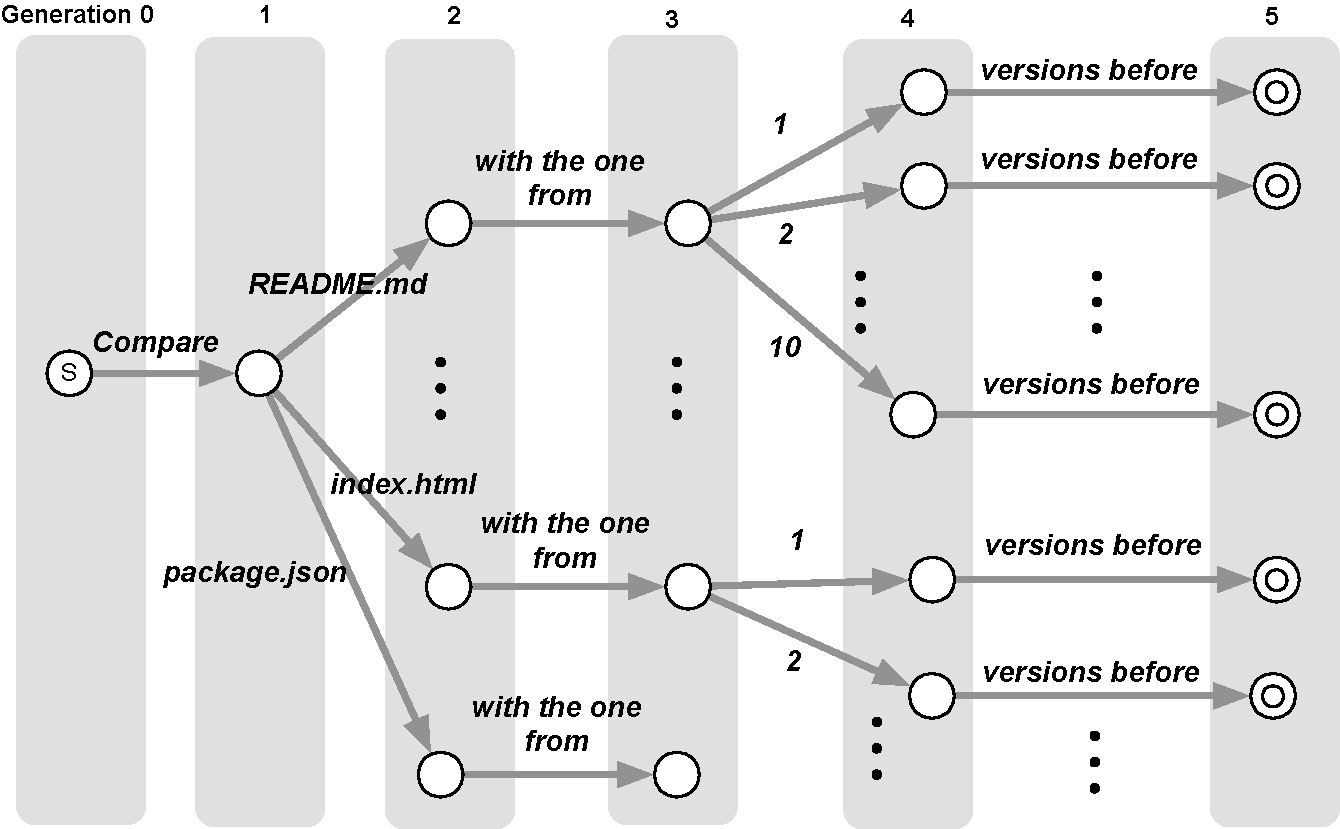
\includegraphics[width=85mm,bb=0 0 643 398]{figures/gentree1.pdf}
\caption{Generating a text tree from a state transition machine.}
\label{gentree1}
\end{figure}

\subsubsection{Generate-and-Filter}

Generating all the texts in this way before finding matched strings is
inefficient, because the amount of generated texts can easily become huge.
Instead, the system performs the patter matching as soon as a text is generated,
for saving time and memory.

``Generate-and-test''\footnote{
  {\sf http:{\slash}{\slash}en.wikipedia.org{\slash}wiki{\slash}Generate\_and\_test}
}
is a simple and effective strategy used for solving puzzles.
For example,
the ``8-Queen'' problem can be solved simply by
generating all the possible queen layouts and checking if
two or more queens are laid out on the same row, column, or diagonal line.
Although this strategy is simple, the cost of
generating all the possible solutions is prohibitive, since
the solution space of the 8-Queen puzzle is $8^8 = 16,777,216$,
which is not a small amount even for today's computers.

To solve this problem,
controlling the generation part from the testing part is effective.
In the 8-Queen problem,
whenever the testing part finds two queens in the same row or column,
it can tell the generation part to
give up current layout in the early stage and proceed to the next layout.

Similarly in our case,
it is not efficient to perform the matching operation
after generating all the texts from the regular expression,
and it is better to calculate the matching
at the time of generating each text.
We call it the \qit{generate-and-filter} strategy,
and implemented the algorithm in {\EH}.
Unlike simple puzzle problems where
conditions are strict and finding one solution is enough,
our goal is to find help description strings
that fits the query pattern while allowing errors.
For this goal,
the system should perform approximate pattern matching
without sacrificing processing speed.
%
We could implement flexible generate-and-filter by using a simple and efficient
approximate pattern matching algorithm based on the ``shifter algorithm''.

\subsubsection{Approximate pattern matching by shifter algorithm}

The ``shifter algorithm''\cite{Wu:1992:FTS:135239.135244}
is a simple and efficient
text search algorithm that has interesting features
not found in more common pattern matching algorithms like
KMP\cite{KMP}, Boyer-Moor\cite{Boyer:1977:FSS:359842.359859}, etc.

When a user wants to find a word \sqsf{README} in a text,
he can use a patter matching state machine like below,
where the gray circle denotes that the state is active.

\begin{figure}[h]
  \centerline{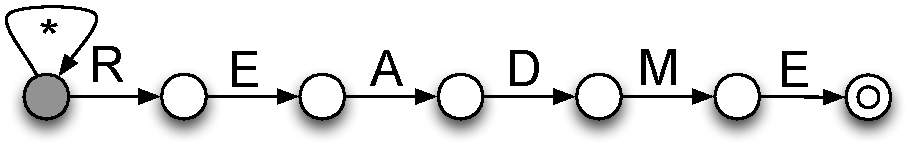
\includegraphics[width=50mm,bb=0 0 439 73]{figures/readme1.pdf}}
  \caption{A state machine for \qsf{README}.}
  \label{readme1}
\end{figure}

Initially, only the leftmost node is active, but when the
state machine receives \sqsf{R}, both the first and the second node become active,
and the activation state will change to the following pattern.

\begin{figure}[h]
  \centerline{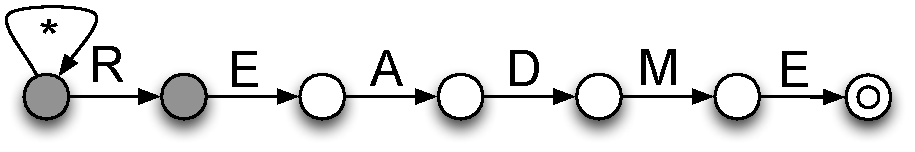
\includegraphics[width=50mm,bb=0 0 439 73]{figures/readme2.pdf}}
  \caption{After receiving \qsf{R}.}
  \label{readme2}
\end{figure}

When \sqsf{README} is given to the state machine,
the rightmost node becomes active.
%
%\begin{figure}[h]
%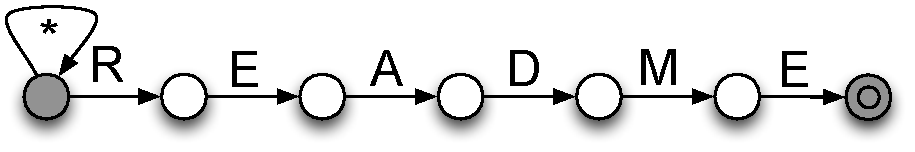
\includegraphics[width=60mm,bb=0 0 439 73]{figures/readme3.pdf}
%\caption{After receiving \qsf{README}.}
%\label{readme3}
%\end{figure}

Although this state machine is a nondeterministic finite state automata (NFA),
only 7 bits are required to represent the active/inactive states of the nodes,
meaning that the whole states can be represented by a single integer value.
Also,
the state transition can be calculated by a simple combination of
logic and bit shift operations.

\subsubsection{Approximate pattern matching using shifter algorithm}

The state machine shown in Figure \ref{readme1} can accept only one pattern
(\sqsf{README}), but
it can be easily expanded to detect texts that contain a word
similar to the pattern (e.g. \sqsf{REEDEE}).

%   *  ** 
%  risto rante
%  restaurant
% \begin{figure}[htb]
%   \centerline{
\includegraphics[width=30mm,bb=0 0 104 51]{figures/readme-mismatch.pdf}}
%   \caption{Matching error between \qsf{README} and \qsf{REEDEE}.}
%   \label{readme-reddy-mismatch}
% \end{figure}

Adding three more rows of states to Figure \ref{readme1}, we can perform more
flexible pattern matcher which can accept strings with
0 to 3 matching errors.

\begin{figure}[htb]
  \centerline{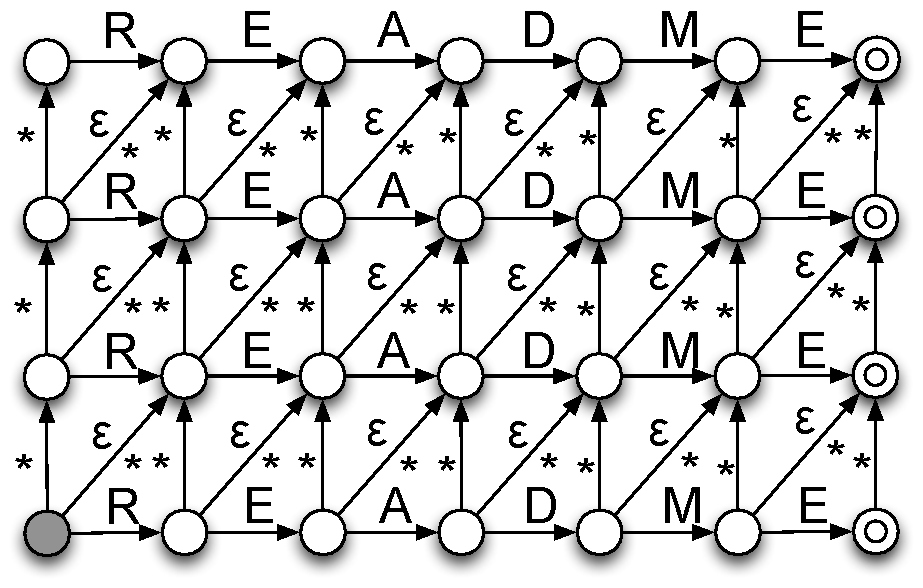
\includegraphics[width=60mm,bb=0 0 443 282]{figures/readme-ambig.pdf}}
  \caption{A pattern matcher accepting 0-3 errors.}
  \label{shifterambig}
\end{figure}

Figure \ref{shifterambig} shows a state machine that can detect a string
that matches \sqsf{README} with 0 to 3 mismatches.
Each additional row of nodes represents a matcher with one error,
two errors, and three errors, respectively.
Vertical and diagonal transition edges are added to allow
transitions based on spelling errors.

Initially, only the bottom-left node is active.
When a character other than \sqsf{R} is detected, 
the transition labeled \sqsf{*} (wildcard) is activated,
and connected nodes become active.
At the same time, links labeled as ``$\epsilon$''
is also activated without any input character.
With these additional links, this expanded machine can detect a text which
matches \sqsf{README} with 0 to 3 errors.

\begin{figure}[htb]
  \centerline{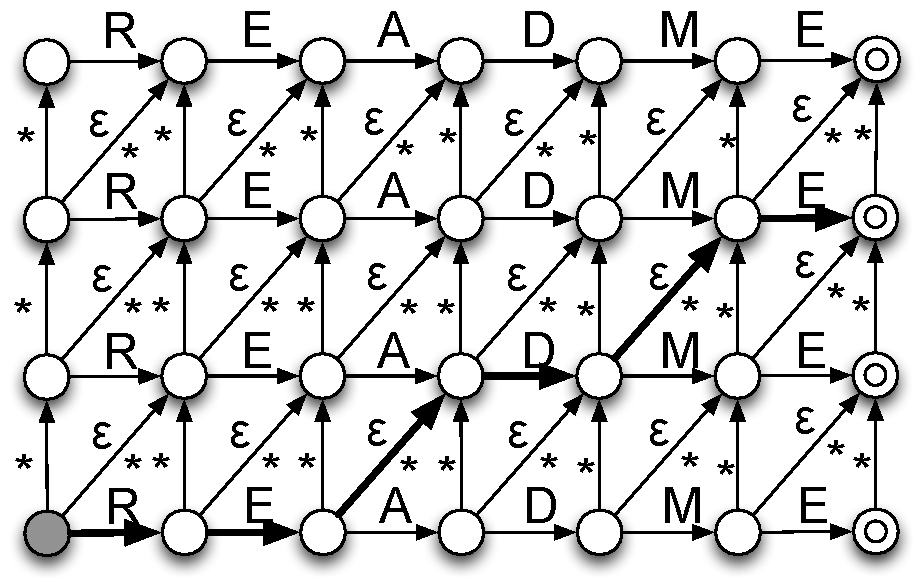
\includegraphics[width=60mm,bb=0 0 443 282]{figures/readme-reedee.pdf}}
  \caption{Accepting \sqsf{REEDEE}'' using a matcher for \sqsf{README}.}
  \label{readme-reedee}
\end{figure}

The transition of active nodes while reading
\sqsf{REEDEE} is shown in Figure \ref{readme-reedee}.
After reading \sqsf{REEDEE},
only the upper-right node becomes active,
denoting that \sqsf{REEDEE} matches
\sqsf{README}'' with 2 matching errors.

The state transition shown in 
Figure \ref{readme-reedee} looks complicated, but
the matching state can be represented by only four integer variables, and
the matching algorithm can be implemented efficiently.

\subsubsection{Using the matcher for generate-and-filter}

We can use this approximate pattern matcher while generating
help texts by traversing the state transition machine.
%
Every time a new node is generated by traversing an edge,
matching state is calculated and stored in the generated node.
The status pattern is calculated from the status pattern
stored in the preceding node and the string associated with the edge.

\begin{figure}[htb]
  \centerline{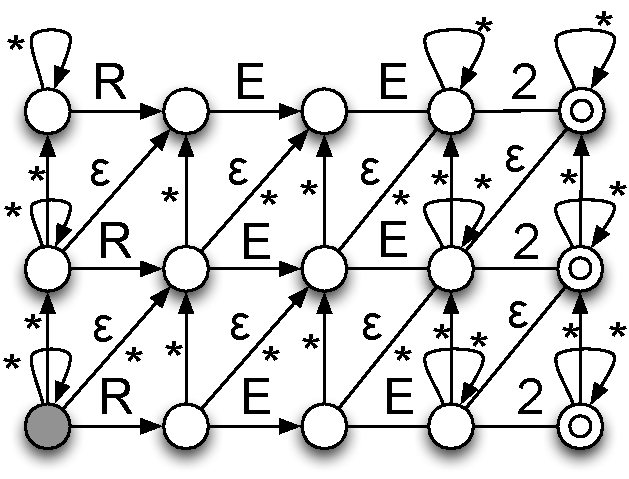
\includegraphics[width=50mm,bb=0 0 302 230]{figures/RE_2.pdf}}
  \caption{A pattern matcher for \sqtt{REE 2}.}
  \label{RE_2}
\end{figure}

\begin{figure*}[bth]
\centerline{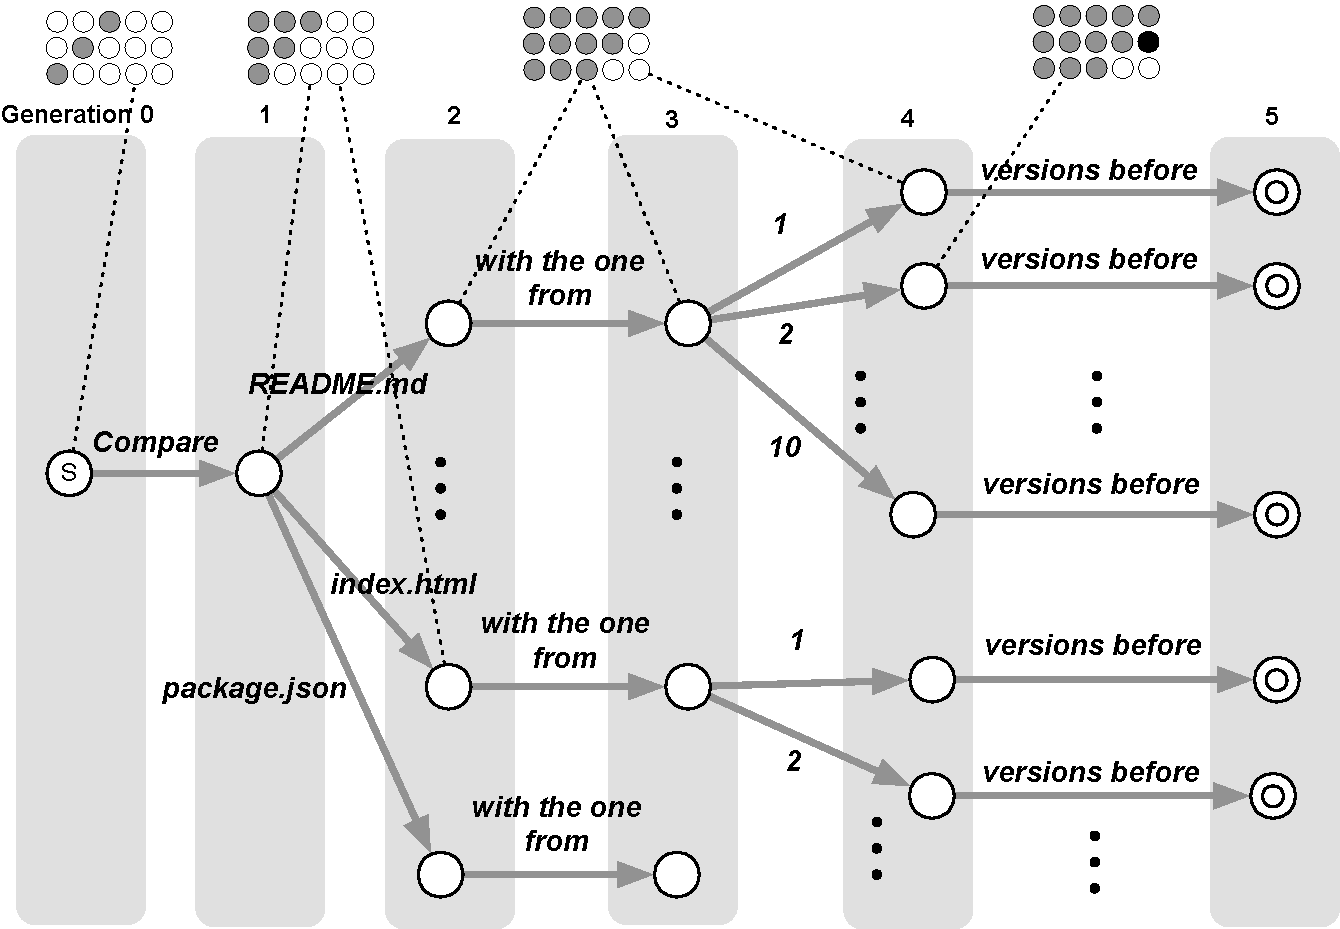
\includegraphics[width=110mm,bb=0 0 643 446]{figures/gentree2.pdf}}
\caption{Matching statuses for \sqtt{REE 2} associated with text generation nodes.}
\label{gentree2}
\end{figure*}

Figure \ref{RE_2} shows the matcher for \sqtt{REE 2}\footnote{
  A space (\qtt{ }) in the input is treated as a wildcard character.
},
and Figure \ref{gentree2} shows how the matching status is calculated while the
description strings are generated from the state transition machine
shown in Figure \ref{statemachine1}.
The matching status at each node is calculated from the matching status
stored in the parent node and the string associated with the edge.
For example, when the system generates the string
\qsf{Compare README.md with the one from 2 versions before},
the matching status is calculated from the status data at the previous node at
\qsf{Compare README.md with the one from 2}, and
the system can tell that it matches \qtt{REE 2} with one matching error,
as soon as the string is generated.

The system is keeping the list of generated strings
which match the pattern with zero to three errors
and it displays the list with minimal number of errors
when generating menu entries.
% 
Since the pattern matching operation is performed at the time of text generation,
the whole generate-and-filter calculation is quick.

% Although current version of ExpandHelp is implemented in MacRuby,
% the user can always get the result within 1 second.
% A portion of the help data in Ruby is shown in Figure \ref{helpdata}.

% \begin{figure*}[bt]
% \centerline{\includegraphics[width=146mm]{figures/04ad7dee5679450e5390821745b5a0b7.png}}
% \caption{A portion of the help data in Ruby.}
% \label{helpdata}
% \end{figure*}

\subsection{Sharing the database on the Web}

The data used in {\GH} are represented as ``{\SB}'' documents
shown in Figure \ref{scrapboxpage}.
%
{\SB} is a general-purpose real-time Wiki system for data sharing.
{\SB} users can edit the contents of Wiki pages directly
on Web browsers just like using text editors.

% \begin{figure}[htb]
% \begin{verbatim}
% \end{verbatim}
% % \centerline{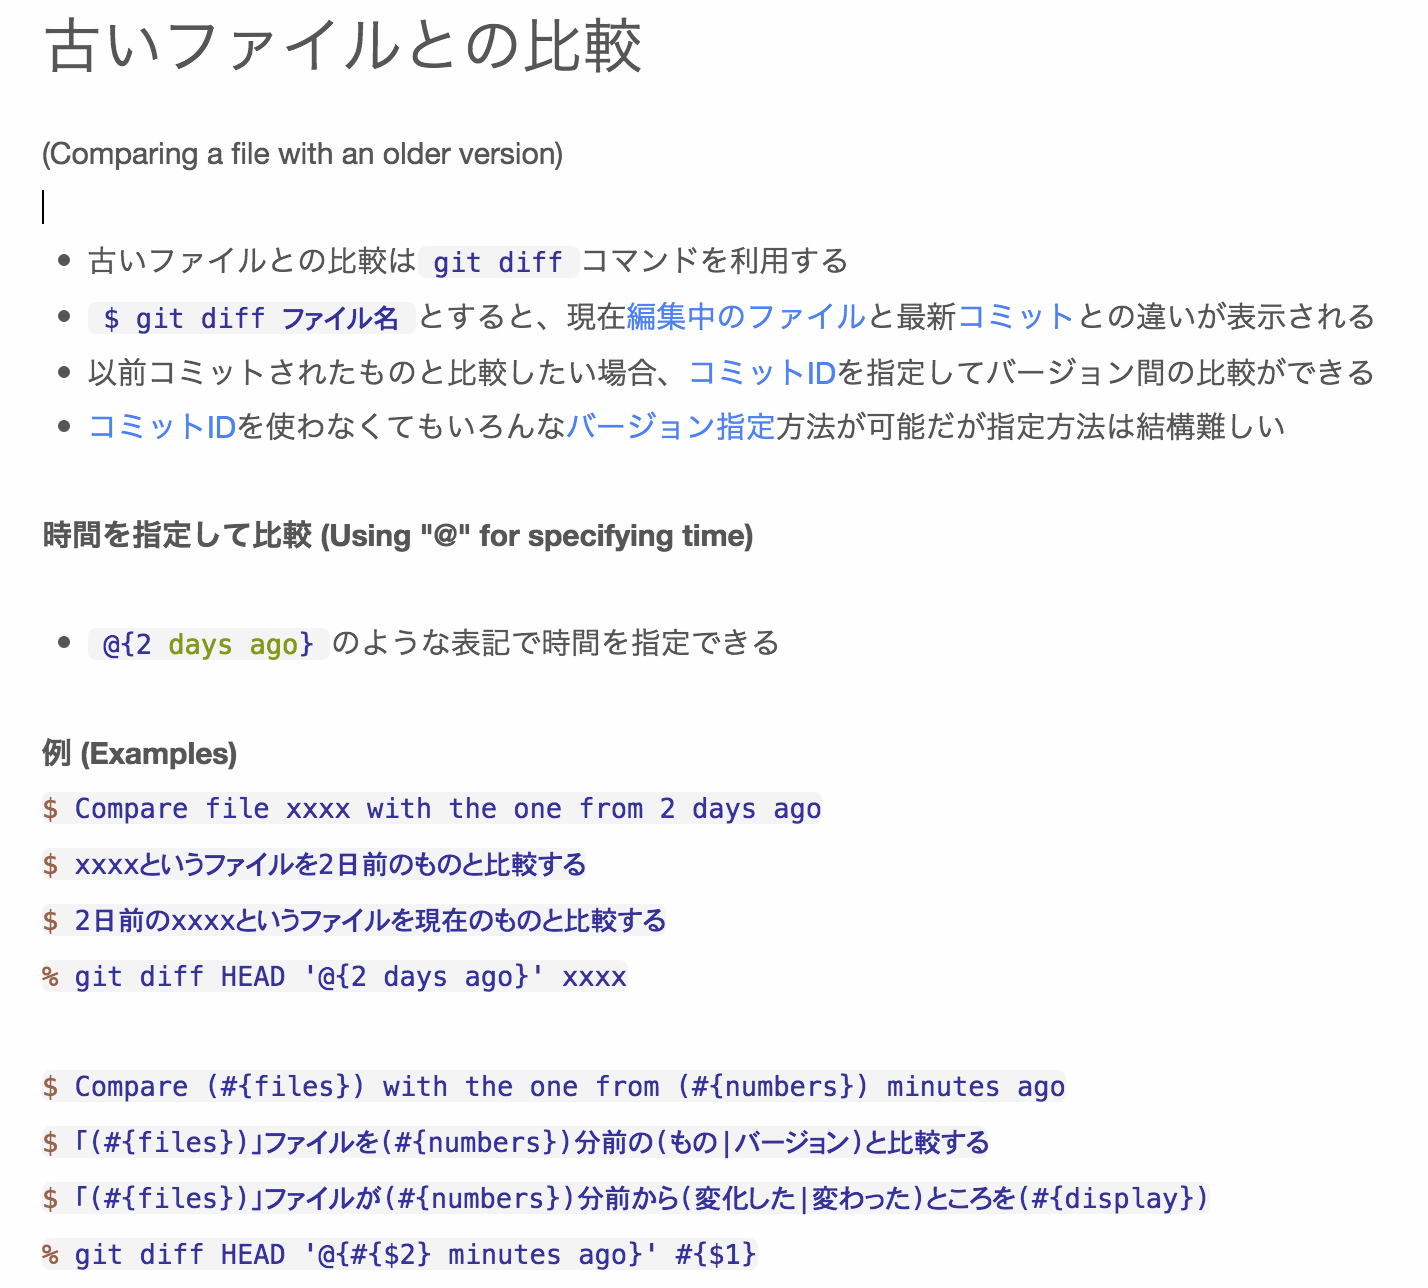
\includegraphics[width=100mm,bb=0 0 1428 1288]{figures/scrapbox1.png}}
% \centerline{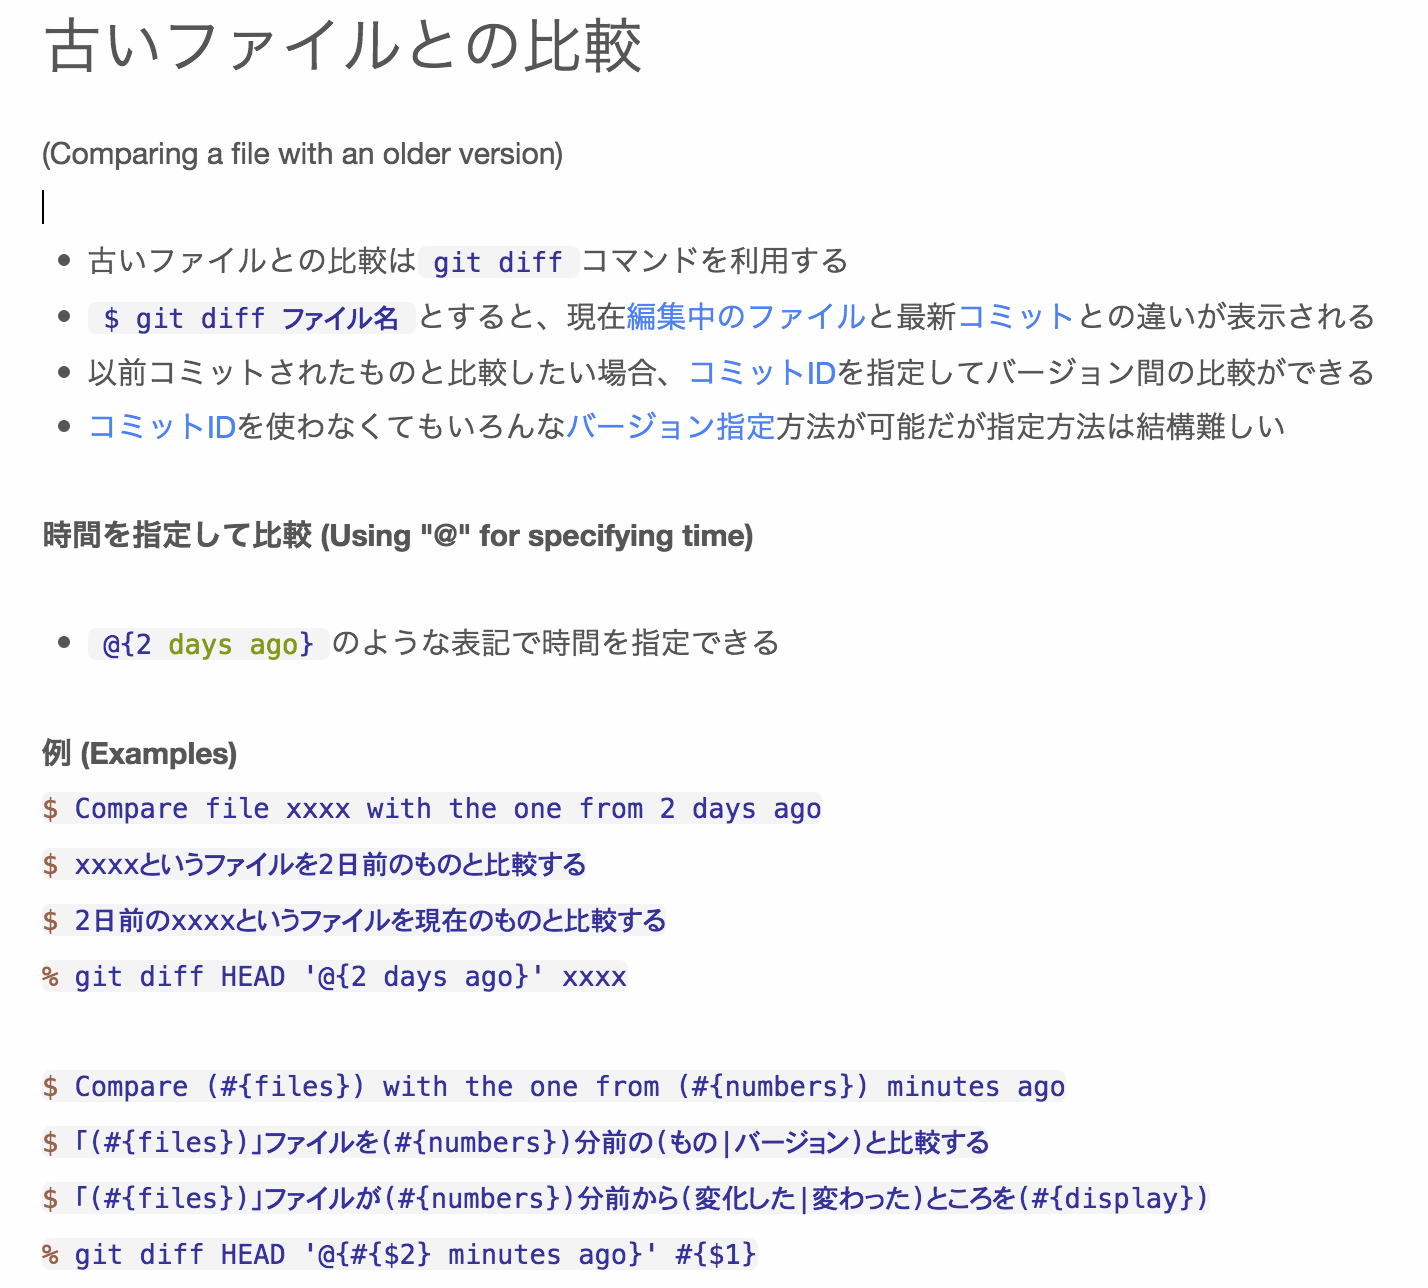
\includegraphics[width=100mm,bb=-50 -50 1000 900]{figures/scrapbox1.png}}
% \caption{A {\SB} page for \tt{git diff}.}
% \label{xxxxx}
% \end{figure}

This page shows how to use \sqtt{git diff}, and
the page contains command specifications in {\EH} format
in addition to the documentation.

% Specs and command lines are specified with a special symbol, and
% all other documents can be written just like standard manuals and help documents.

Usage examples are often shown on documents and manuals like Unix man pages,
but they cannot be used as the database of an online help system.
On the other hand,
a {\SB} document contains both the manual document and the help database
in the same place, just like
writing a source code and the document in the same place
under the ``Literate Programming''\footnote{
  \ssf{https:{\slash}{\slash}en.wikipedia.org{\slash}wiki{\slash}Literate\_programming}
} style.

Also, since the database is on the Wiki page, any member of the
Wiki can correct the document or add additional {\GH} specifications.
When a user could not get a good support from {\GH}, he can add
{\EH} specifications to the {\SB} document himself
so that he and other people can get better support
from {\GH} next time.

\section{Related Work}

\subsection{Intelligent help systems}

There have long been many researches on
intelligent help systems\cite{Delisle:2002:UIH:606412.606415},
but few number of projects seem to be going on these days,
maybe because now we can use the Internet for getting intelligent help from
real people,
either by searching existing Web pages or 
by asking in user forums like StackOverflow\footnote{
  \textsf{https://stackoverflow.com/}
}.
Information on the net is rich these days, and we can easily
find somebody who can give good answers to our questions.
This is a good news, but 
asking many trivial questions on the net is not considered to be a
good manner, and
using a powerful and flexible local help system like {\EH} is
preferable most of the time.

\subsection{Input Methods}

Text input systems for non-English languages are widely used
in the world,
and they are called as ``Input Methods'' (IMs).
%
Many research and development on IMs have been going on for years, and
people are using them every day for entering texts in their mother language.
Figure \ref{gyaim} shows an example of a Japanese IM.

\begin{figure}[H]
  % \includegraphics[width=8cm,bb=0 0 976 670]{figures/nyuuryoku-ime.png}
  \centerline{\includegraphics[width=8cm,bb=0 0 976 670]{figures/nyuuryoku-ime.png}}
  \caption{An IM for Japanese text input.}
  \label{gyaim}
\end{figure}

IMs are one form of translation systems that convert one
expression (pronunciation, character shape, etc.)
into a textual form of a language.
In the above example, the pronunciation ``kanji''
is used for getting ``漢字''.

IMs are very popular in the modern computing environment in the world
and it is very common for people to 
use translation systems for using computers.
%
The behavior of {\GH} is similar to conventional IMs, and
integration of multiple IM-like systems should be challenged in the future.

\subsection{Text and code completion}

On text editors and Unix shells,
``text completion'' feature has been available for a long time.
%
When a user types the TAB key after typing \sqtt{la} on the Unix shell,
\sqtt{latex}, \sqtt{last}, and other Unix commands are shown as candidates.
When a user types \sqtt{ls RE} and types the TAB key,
the shell checks the directory, find the \stt{README.md} file, and
replace the user's input with \sqtt{ls README.md}.
This behavior is called ``text completion'', and many variations of
this idea have been proposed and adopted in command shells and text editors.

% User's history data can also be used for the completion function.
% The Reactive Keyboard\cite{ReactiveKeyboard}
% accumulates the user's command history and use the data
% for predicting the user's next input.

Gitsome\footnote{\textsf{https:{\slash}{\slash}github.com{\slash}donnemartin{\slash}gitsome}}
helps {\GIT} users by
dynamically showing possible arguments and related manuals on the Unix shell,
just like {\GH} does.
The goal of Gitsome is almost the same as {\GH} and we agree with its concept,
but Gitsome does not support flexible approximate matching and
help data sharing.

\subsection{Smart IDEs}

Integrated Development Environments (IDEs) are widely used for
software development, and
many smart IDEs for suggesting codes have been proposed recently.

Little's system\cite{Little:2006:TKC:1166253.1166275}
generates a complete JavaScript code snippet from keyword fragments
give by users.
For example, a code snippet
\sqtt{ActiveDocument.PageSetup.LeftMargin = InchesToPoints(2)}
can be generated from keywords like
\sqsf{left},
\sqsf{margin},
\sqsf{inches},
and \sqsf{2}.
The system generates the code using a template database and heuristics
designed for the target system.
It is useful for a specific environment, but
users of the system cannot modify the algorithm or the database
even when no good suggestion was found.

% キーワードの羅列からコマンドを作成するという考えはとても正しいと思うが、実装がいかがなものか?
% キーワードぐらいは思い出せるプログラマが対象になっている
% 「margin」とか「left」とかいう単語は思い出す必要がある
% 「ちょっと字下げ」とか言っても駄目
% キーワードが違ってると駄目?
% いろいろズルをしてるようだ
% [[ActiveDocument]]はよく出てくるので特別扱いしているとか
% ステミングをしている
% ``the'' ``to'' などは捨ててるのだろう
% そもそもリカーシブな検索アルゴリズムにかなり無理がありそう
% テンプレートを作るのは大変ではないのか?

% https://www.youtube.com/watch?v=93vZAmLyOQY
AnyCode\cite{Gvero:2015:SJE:2814270.2814295} is another system
that generates a complete code snippet from the user's
input in natural language.
AnyCode can handle synonyms database like ``make'' == ``create'',
but approximate matching is not supported and
users cannot modify the help database.

% 曖昧検索はできず、かなりキーワードを指定する必要はある

% [anyCode]というシステム。自然言語キーワードを入力するとコードスニペットが表示される。
% [[copy fileA fileB]]みたいなキーワードから[[FileUtil.copyFile(new File(fileA), new File(fileB))]]みたいなコード候補を生成する
% [自然言語処理]を行なっている
% [https://github.com/tihomirg/nlpcoder/tree/noola GitHub]
% 曖昧検索はできない
% 真面目に自然言語を入れる必要がある
% `123`みたいなパラメタは使えるか?
% 使えると思うが例には出てこない
% コードの説明文は出ない?
% FileUtil.copyFile(new File(fileA), new File(fileB)) と言われても、どちらが新しいファイルなのかわからない

Active Code Completion\cite{Omar:2012:ACC:2337223.2337324}
is another code completion system for the Eclipse IDE.
A database called \textit{palette} are used for code completion and coding support
for Java classes.
When a user wants to write a code for drawing a rectangle in purple,
the user should just tell ``purple'' to the system,
and the system shows the user a color selection window
as well as the Java code for drawing a purple rectangle.
This is a useful feature for the user to write a code including selecting
a color, but palettes are difficult to create, and should be provided
as IDE plugins.
% [/ palette] と呼ばれるテンプレートを用意して[IDE]でのコード補完をサポートする
% `getDefaultColor()` を定義したいとき`purple`と入力すると、それに対応した候補が提示されるとか
% 普段使ってる環境で有益な候補が表示されると嬉しいだろうと言っている
% [[コメント]]
% [Jun Kato.icon]
% > Active code completionも思い出しました。型ごとに適した入力インタフェースを出すコード補完インタフェースのnn提案です。確か。
% [増井俊之.icon]
% IDEでどういう機能が欲しいかサーベイして設計したことになっている
% 色選択と正規表現のためのコード生成をサポートした例が紹介されている
% 一般的な補完コマンド起動によって呼び出されるようだ
% サポートウィンドウはHTML5で生成する
% しかし両者とも[/palette]の作成はかなり大変である
% 普通のユーザが作れるようなものではない
% [* 作成がすごく大変]で、[* 特定のIDEでしか使えない]という問題があると思う

Han's Abbreviation Completion system\cite{Han:2009:CCA:1747491.1747530}
can generate a code snippet from abbreviation strings give by the user.
For example, a code snippet like \sqtt{chooser. showOpenDialog()}
can be generated from strings like
\sqsf{ch} and \sqsf{opn}, using the code database and HMM.
It can be very useful as a shorthand for handling long names,
but users should have a vague knowledge about the correct names
(e.g. \sqtt{chooser}, \sqtt{dialog}),
and large code example corpus should exist before being able to
create the database.
{\EH} database can be created by hand at the time of the system development
and no corpus is required.

% [HMM]を使って正しいコードを予測して提示する
% `ch opn`みたいなテキトーな入力から`chooser.showOpenDialog()`みたいな正しいコードが候補に出る
% コードデータベースを解析
% [[コメント]]
% [増井俊之.icon] 2018/3/23 18:53
% コードのほんの一部を指定すると正しく予測されるというのは面白い
% HMMってそういうのに使えるのね
% しかし[* 関数名とか全然覚えていないときは使えないだろう]
% [語彙問題]が解決できてない
% だとすると高速入力の役にはたつが、何もかもわからない人をサポートはできない
% 用例データが存在しない場合も使えない
% [IDE]でしか使えない
% [Cyrus Omar: Active code completion]で参照されている

\subsection{Using cloud data for development}

% 他人の情報利用する系
% コード共有、コンパイルエラー共有

Many systems support sharing users' development experiences on the web so that
they can be used on the developers' IDE.

Using BluePrint\cite{Brandt:2010:EPI:1753326.1753402}
as a plugin for Adobe Flex Builder,
users can search sample codes from the Web and use it immediately.
%   サンプルコードをすぐ参照して利用できる[IDE]
%
HelpMeOut\cite{Hartmann:2010:OPS:1753326.1753478} tells users
how to handle compile errors,
based on the people's experiences of handling compile errors.
%
Resources on the net are precious, and such data can be
easily incorporated to {\EH} databases.

%= 他人のヒストリを使ってコンパイルエラー対処法をサジェスト

% \subsection{Literate Programming}
% 
% Literate Programming\cite{Knuth}
% 
% 参考文献にすることはないか
% 
% JavaDoc
% Jupyter
% Eve

\section{Discussions}

\paragraph{Applications of ExpandHelp}

Since the translation mechanism of {\EH} is simple and flexible,
it can be used for a wide range of application domains where
intelligent help is required.
{\EH} is actually used as the help page for
one of our Web services, hoping that
novice users can easily find the feature they need.
When a user submits a query that includes vocabularies
not in the {\EH} document,
we are able to add them to the {\SB} database easily.

Figure \ref{mac1} and Figure \ref{mac2} shows how
{\EH} can be used as a launcher for MacOS.
Like {\GH}, users can execute concrete commands only by
showing small fragments of their intentions to the system.

\begin{figure}[h]
  %\centerline{\includegraphics[width=8cm,bb=0 0 397 247]{figures/clock.png}}
  \centerline{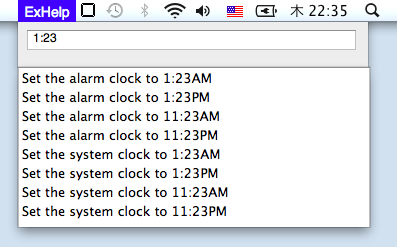
\includegraphics[width=8cm,bb=0 0 300 200]{figures/mac1.png}}
  \caption{Using {\EH} in the menu bar of MacOS.}
  \label{mac1}
\end{figure}

\begin{figure}[h]
  %\centerline{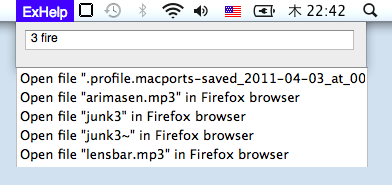
\includegraphics[width=8cm,bb=0 0 392 185]{figures/mac2.png}}
  \centerline{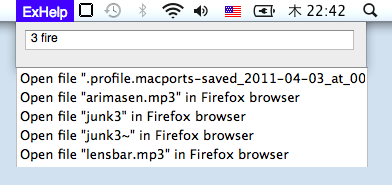
\includegraphics[width=8cm,bb=0 0 300 130]{figures/mac2.png}}
  \caption{Using {\EH} in the menu bar of MacOS.}
  \label{mac2}
\end{figure}

\paragraph{Order of command and arguments}

Using a command shell,
users have to enter a command first and enter options and arguments after that.
Using a GUI desktop,
users can right-click a data icon to show a menu,
and select what he wants to do from the menu.
Switching between command-oriented usage pattern and
data-oriented usage pattern is sometimes confusing.
Using {\EH}, users can find what they can do
either by specifying commands or by specifying data, 
without worrying about the order.

\paragraph{Usage of regular expressions}

An advantage of using a regular expression is that
it is fairly easy for users to write description texts.
People can easily write a help description like
\sqtt{(Start|Run) Firefox browser}
without having a knowledge of automata or formal grammar.
We can use arbitrary texts for the database of {\EH}.
For example,
we can collect hundreds of books titled ``Windows tips'' from the market
and convert all the title of the tips into help data of {\EH}.

\section{Conclusion}

We proposed the ``translation paradigm'' for bridging the gap between
users' intention and actual operations.
%
We have introduced a general-purpose flexible framework {\EH}
that can translate fragments of user's vague intentions into
concrete command strings required to control computers and
other complex artifacts.
We showed the principles and applications of {\EH} by using it
for {\GH}, a help system for supporting {\GIT} users
based on the shared database that any user can edit to share
translation knowledge between users.
%
{\EH} framework is useful for any kind of systems that need
some kind of user support, and we are planning to use it
for various applications and Web services in the future.

% Unlike existing smart IDEs for supporting programming tasks,
% {\EH} framework can be used in wide range of situations
% where translation-based help is required.
% 
% Using the powerful and flexible help system ``{\EH}''
% constructed on the generate-and-filter algorithm, where
% the system generates all the possible expressions of
% help entries expanded from regular expressions,
% while the output expressions are filtered by search keywords using
% an efficient approximate pattern matching algorithm.
% 
% Since the data format is simple and the search algorithm is fast and flexible,
% developers can easily publish useful help data, while
% users can have bigger chances of finding an appropriate
% data from vague knowledges.

% References must be the same font size as other body text.
\bibliographystyle{SIGCHI-Reference-Format}
\bibliography{paper}

\end{document}
